\documentclass[a4paper,12pt]{article}
\usepackage{amsmath}
\usepackage{bm}
\usepackage{amsfonts}
\usepackage{amssymb}
\usepackage{setspace}
\usepackage{helvet}
\usepackage{graphicx}
\usepackage{setspace}
\usepackage{listings}
\usepackage[style = numeric, backend = bibtex]{biblatex}
\graphicspath{ {./images/} }

\newcommand{\set}[1]{\mathcal{#1}}
\newcommand{\operation}{\bigotimes}
\newcommand{\matrx}[1]{\bm{#1}}
\newcommand{\vectr}[1]{\textbf{#1}}
\newcommand{\real}{\mathbb{R}}
\newcommand{\natral}{\mathbb{N}}
\newcommand{\integers}{\mathbb{Z}}
\newcommand{\italic}[1]{\textit{#1}}
\newcommand{\rrank}[1]{rk_{row}(\matrx{#1})}
\newcommand{\crank}[1]{rk_{col}(\matrx{#1})}
\newcommand{\nexteq}{\refstepcounter{equation}\theequation}
\newcommand{\dett}[1]{\text{det}(\matrx{#1})}
\newcommand{\mdett}[1]{\text{det} \left ( #1 \right )}
\newcommand{\lcomb}[1]{\sum_{i = 0}^{k} {#1} \vectr{v}_i}
\newcommand{\vecspace}[1]{#1}

% new environments 
% recto  inverso 
% set book class to one sided
% add chapter levels
% new environment / draft notes / if then else draft = 1 / check the internet for prior examples

\doublespacing
\setstretch{1.5}

\newtheorem{definition}{Definition}[section]
\newtheorem{proposition}{Proposition}[section]
\newtheorem{theorem}{Theorem}[section]

\newenvironment{code}{\ttfamily\\}{\\}
\newenvironment{scode}{\vspace{10pt} \begin{code}}{\vspace{10pt} \end{code}}

\addbibresource{sources/sourcesnew.bib}

\begin{document}
	\vspace*{\fill}
	\begin{center}
		
\includegraphics[scale = 0.15]{brunel logo.png}
		
		\vspace{1cm}
		\Large{Department of Mathematics, College of Engineering, Design and Physical Sciences, Brunel University}
		
		\vspace{1cm}
		\Large{Mathematics (MMath)}
		
		\vspace{1cm}
		\large{Academic Year 2022 - 2023}
		
		\vspace{1.5cm}
		\LARGE{\bf Applications of Genetic Algorithms}
		
		\vspace{1cm}
		\large{By David Blair}
		
		\vspace{0.1cm}
		\large{Supervisor: Dr Simon Shaw}
	\end{center}
	\vspace*{\fill}
	\newpage
	
	\tableofcontents
	
	\section{Vector Space}
	% vector space introduction
	A vector space is an algebraic structure that consists of a set of vectors and two operations defined on these vectors: vector addition and scalar multiplication. Vectors can be added together and multiplied by numbers, called scalars. The operations of vector addition and scalar multiplication must satisfy a set of axioms, which ensure that the resulting vectors remain within the vector space. It will be helpful to describe a vector space by first explaining the concept of a set and a group. 
	
	% set definition
	A set is a collection of mathematical objects such as numbers, lines or potentially other sets. They were first formalised by George Cantor in 
	1895 \cite{def_set_cantor} as being either infinite or finite and containing distinct elements. 
	% group definition
	\begin{definition}\normalfont
		Let $ \mathcal{V} $ be a set and $ \operation $ denote a binary operation between elements of this set such that $ \operation : \set{G} \times \set{G} \rightarrow \set{G} $. $G := (\set{G}, \operation)$ is called a group  \cite{def_group} if the following conditions are met:
		\begin{enumerate}
			\item (Closure) The binary operation between any two elements of the set will result in an element which is also part of the set: $ \operation : \forall x,y \in \set{G} : x \operation y \in \set{G} $.
			\item (Associativity) The order in which group operations are performed on a set of elements is irrelevant: $ \forall x, y, z \in \set{G} : (x \operation y) \operation z = x \operation (y \operation z) $.
			\item (Neutral Element) A neutral element in a set is an element that, when combined with any other element in the set using the group operation, results in the same element: $ \exists e  \in \set{G} \forall x \in \set{G} : x \operation e = x$ and $ e \operation x = x $.
			\item (Inverse Element) The inverse of an element in a set is an element that when combined with the original element using the group operation, results in the neutral element. It allows for the reversal of the group operation: $ \forall x \in \set{G} \exists y \in \set{G} :  x \operation y = e$ and $ y \operation x = e $, where $ e $ is the neutral element. We can denote the inverse of an element $ x $ as $ x^{-1} $.
		\end{enumerate}
	\end{definition}
	
	% relevence of groups 
	Groups are very important in many areas of mathematics. Their rigorous and formal definition means that, if something is found to be a group, its properties can be better understood in the specific context in which it is relevant.
	% example of group 
	% ammend: general linear group being in italic / reference from the book / regular (invertible) not regular invertible
	An example of a group is the general linear group. This is the set of regular invertible matrices $ \matrx{A} \in \real^{n \times n} $ where the group operation is matrix multiplication. The inverse elements would be the inverse of the matrix and the neutral element would be the identity matrix. However, the order in which the group operation is performed will affect the result i.e $ \matrx{AB} \ne \matrx{BA} $. 
	% definition of an abelian group
	Given a group $ G $, if the order in which the group operation is performed does not matter i.e. $ \forall x, y \in \set{G} : x \operation y = y \operation x $, then $ G = (\set{G}, \operation) $ is known as an \italic{Abelian group} (commutative). An example of this would be $ (\integers, +) $, the set of all integers under the addition operation.
	
	
	% definition of a vector space
	A vector space \cite{def_vector_space} is a special type of group with some additional conditions. 
	
	\begin{definition}[Vector Space]
		\normalfont A real-valued $\italic{vector space}$ $V = (\set{V}, +, \cdot)$ is a set $\set{V}$ with two operations:
		\begin{align}
			+: \set{V} &\times \set{V} \rightarrow \set{V} \hspace{10pt} (\text{Inner Operation}) \\
			\cdot: \real &\times \set{V} \rightarrow \set{V} \hspace{10pt} (\text{Outer Operation})
		\end{align}
		where:
		\begin{enumerate}
			\item $(\set{V}, +)$ is an Abelian group
			\item (Distributivity) The outer operation can be ``Distributed'' across elements either before or after the inner operation has occurred: 
			\begin{enumerate}
				\item $\forall \lambda \in \real, \vectr{x}, \vectr{y} \in \mathcal{V}: \lambda (\vectr{x} + \vectr{y}) = (\lambda \cdot \vectr{x} + \lambda \cdot \vectr{y})$
				\item $\forall \lambda, \psi \in \real, \vectr{x} \in \set{V}: (\lambda + \psi) \cdot \vectr{x} = \lambda \cdot \vectr{x} + \psi \cdot \vectr{x}$
			\end{enumerate} 
			\item Associativity (outer operation): $\forall \lambda, \psi \in \real, \vectr{x} \in \set{V}: \lambda \cdot (\psi \cdot \vectr{x}) = (\lambda \psi) \cdot \vectr{x}$
			\item Neutral element with respect to the outer operation: $\forall \vectr{x} \in \set{V}: 1 \cdot \vectr{x} = \vectr{x}$
		\end{enumerate}
		\label{def:vector_space}
	\end{definition}
	It is also the case that non-real valued vector spaces are permitted. 
	
	% generalisation of a vector
	We commonly think of vectors as being mathematical objects with both direction and magnitude. However, these are only geometric vectors. More generally, any set of objects which follows the definition of a vector space is known as a vector. For example, polynomials of the same degree are also vectors. Two can be added together, resulting in another polynomial of the same degree and they can be multiplied by a scalar $ \lambda \in \real $ which again results in another polynomial. 
	
	% ammend: add some more details here about how the specific examples fit into the axioms of a vector space. You should also include an example of a finite dimensional and infinite dimensional situation.
	
	
	% begin linear independence
	\section{Linear Independence}
	Linear independence \cite[page 40]{mml_book} is a property of a set of vectors which describes whether there is any redundancy with respect to the linear combinations of these vectors. 
	% definition of linear combination
	\begin{definition}[Linear Combination] \cite[page 40]{mml_book}
		\normalfont	Consider a vector space $\italic{V}$ and a finite number of vectors $\vectr{x}_i,\ldots,\vectr{x}_k \in \italic{V}$. Then, every $\vectr{v} \in \italic{V}$ of the form
		\begin{align}
			\vectr{v} = \lambda_1\vectr{x}_1 + \cdots + \lambda_k\vectr{x}_k =  \sum_{i=1}^{k} \lambda_i\vectr{x}_i \in \italic{V}
		\end{align}
		with $\lambda_1,\ldots,\lambda_k \in \real$ is a $\italic{linear combination}$ of the vectors $\vectr{x}_1,\cdots,\vectr{x}_k$.
		\label{def:linear_combinations}
	\end{definition}
	% base vectors of R^2
	Consider two vectors in $ \real^2 $, $\vectr{e}_1 = (1, 0)^{\top}$ and $\vectr{e}_2 = (0, 1)^{\top}$. It is common to see these written as $ \vectr{i} $ and $ \vectr{j} $ respectively. We can represent any vector in $ \real^2 $ as a linear combination of these two vectors: \\
	\italic{Proof}:
	We can express any vector in $ \real^{2} $ as $ \vectr{v} = (\alpha, \beta)^{\top} $ where $ \alpha, \beta \in \real $. It is the case that $ \matrx{I}\vectr{v} $ = $ \vectr{v} $ for all $ \vectr{v} $. Therefore:
	\begin{align}
		\matrx{I}\vectr{v} = \vectr{v} = \begin{bmatrix}
			1 & 0 \\
			0 & 1 
		\end{bmatrix} \begin{bmatrix}
			\alpha \\
			\beta 
		\end{bmatrix} = \alpha \begin{bmatrix}
			1 \\
			0 
		\end{bmatrix} + \beta \begin{bmatrix}
			0 \\
			1
		\end{bmatrix} = \alpha \vectr{e}_1 + \beta \vectr{e}_2
	\end{align}
	% definition of linear independence
	\begin{definition}[Linear Dependence] 
		\normalfont Consider a vector space $\italic{V}$ with $k \in \natral$ and  $\vectr{x}_1,\cdots,\vectr{x}_k \in \italic{V}$. If there is a non-trivial combination, such that $\vectr{0} = \sum_{i=1}^{k} \lambda_i\vectr{x}_i$ with at least one $\lambda_i \ne 0$, the vectors  $\vectr{x}_1,\cdots,\vectr{x}_k$ are \italic{linearly dependent}. \label{def:linear_independence}
	\end{definition} 
	% definition of linear dependence
	\begin{definition}[Linear Independence]
		\normalfont Consider a vector space $\italic{V}$ with $k \in \natral$ and  $\vectr{x}_1,\cdots,\vectr{x}_k \in \italic{V}$. If only the trivial solution exists, such that $\vectr{0} = \sum_{i=1}^{k} \lambda_i\vectr{x}_i$ with all $\lambda_i = 0$, the vectors $\vectr{x}_1,\cdots,\vectr{x}_k $ are \italic{linearly independent}.
		\label{def:linear_independence}
	\end{definition}
	% example of linear independence through linear combinations
	Lets consider the following set $\set{V}$ of vectors $\vectr{v}_1,\vectr{v}_2 $ and $ \vectr{v}_3$ where (respectively):
	\begin{align}
		\set{V} = \left\{\begin{bmatrix} 1 \\ 2 \end{bmatrix},\begin{bmatrix} -2 \\ -4 \end{bmatrix},\begin{bmatrix} -4 \\ -1 \end{bmatrix} \right\}
	\end{align}
	And let $\vectr{y} \in \real^2$ be any linear combination that can be made from these vectors. Writing this out explicitly with $\alpha, \beta, \omega \in \real$:
	\begin{align}
		\vectr{y} &= \alpha \begin{bmatrix} 1 \\ 2 \end{bmatrix} + \beta \begin{bmatrix} -2 \\ -4 \end{bmatrix} + \omega \begin{bmatrix} -4 \\ -1 \end{bmatrix} \\
		&= \alpha \begin{bmatrix} 1 \\ 2 \end{bmatrix} - 2\beta \begin{bmatrix} 1 \\ 2 \end{bmatrix} + \omega \begin{bmatrix} -4 \\ -1 \end{bmatrix} \\
		&= (\alpha - 2\beta) \begin{bmatrix} 1 \\ 2 \end{bmatrix} + \omega \begin{bmatrix} -4 \\ -1 \end{bmatrix} \\
	\end{align} 
	% intuition behind linear independence 
	What we have shown is that if a vector $ \vectr{y} $ can be represented as a linear combination of $ \vectr{v}_1,\vectr{v}_2 $ and $ \vectr{v}_3 $ then we can represent $ \vectr{y} $ as a linear combination of $ \vectr{v}_2 $ and $ \vectr{v}_3 $. This is because $ \vectr{v}_1 $ is a scaled version of $ \vectr{v}_2 $ and vice versa. 
	% leading into the formal definition 
	More formally:
	
	\begin{align}
		\begin{bmatrix} -2 \\ -4 \end{bmatrix} + 2 \begin{bmatrix} 1 \\ 2 \end{bmatrix} = \vectr{0}
	\end{align}
	
	which following from definition \ref{def:linear_independence} demonstrates that we have a linearly dependent set of vectors.
	\section{Generating Set and Span}
	
	A generating set and the span \cite[page 44]{mml_book} of a set of vectors are concerned with the vector space produced by the linear combination of all the vectors in the set.
	
	% definition of a generating set and span
	\begin{definition}[Generating Set and Span] \cite{def_generating_set_span}
		\normalfont Consider a vector space $\italic{V} = (\set{V}, +, \cdot)$ and set of vectors $\set{A} = \{\vectr{x}_1,\ldots,\vectr{x}_k\} \subseteq \italic{V}$. If every vector $\vectr{v} \in \italic{V}$ can be expressed as a linear combination of vectors of $\vectr{x}_1,\ldots,\vectr{x}_k$, $\set{A}$ is called a generating set of $\italic{V}$. The set of all linear combinations of vectors in $\set{A}$ is called the span of $\set{A}$. If $\set{A}$ spans the vector space $\italic{V}$, we write $\italic{V} = span[\set{A}]$. 
		\label{def:generating_set_span}
	\end{definition}
	
	% generating set of R^2
	Consider the vector space $ V = (\real^{2}, +, \cdot) $ under vector addition and scalar multiplication. Previously we have said that every vector $ v \in V $ can be represented as a linear combination of $\vectr{e}_1 = (1, 0)^{\top}$ and $\vectr{e}_2 = (0, 1)^{\top}$. By definition \ref{def:generating_set_span}, the set of vectors $ \set{B} = \{ \vectr{e}_1, \vectr{e}_2 \} $ is a generating set of $ V $. 
	% span of base vectors of R^2
	On the other hand, the set of two-dimensional vectors $ \real^{2} $ contains all linear combinations of the set $ \set{B} $ meaning that the $ span[\set{B}] = \real^{2} $. In this sense, a generating set and the span of a set are two sides of the same coin.
	\section{Basis}
	
	% reasoning behind a basis
	A basis is concerned with the minimum number of vectors that would be needed to span a particular vector space. 
	% basis definition
	\begin{definition}[Basis] \cite{def_basis}
		\normalfont Consider a vector space $\italic{V} = (\set{V}, +, \cdot)$ and $\set{A} \subseteq \set{V}$. A generating set $\set{A}$ of $\italic{V}$ is called $\italic{minimal}$ if there exists no smaller set (with a lower cardinality) $\set{\tilde{A}} \subseteq \set{A} \subseteq \set{V}$ that spans $\italic{V}$. Every linearly independent generating set of $\italic{V}$  is minimal and is called a $\italic{basis}$ of $\italic{V}$.
		\label{def:basis}
	\end{definition}
	% basis example
	Consider the vector space $ \italic{V} = (\real^{3}, +, \cdot) $. A potential generating set for $ \italic{V} $ is the set $ \set{A} $ where:
	% basis vectors for R^3
	\begin{align}
		\set{A} = \left\{\begin{bmatrix} 1 \\ 0 \\ 0  \end{bmatrix},\begin{bmatrix} 0 \\ 1 \\ 0 \end{bmatrix},\begin{bmatrix} 0 \\ 0 \\ 1 \end{bmatrix} \right\}
	\end{align}
	% informal explanation for a basis
	This is because every vector in $ \real^{3} $ can be represented as linear combinations of the vectors in $ \set{A} $:
	\italic{Proof}: Given a vector $ \vectr{v} \in \real^{3} $:
	\begin{align}
		\vectr{v} = \matrx{I}\vectr{v} = \begin{bmatrix}
			1 & 0 & 0 \\
			0 & 1 & 0 \\
			0 & 0 & 1 
		\end{bmatrix} \begin{bmatrix}
			v_1 \\
			v_2 \\
			v_3
		\end{bmatrix} = v_1 \begin{bmatrix}
			1 \\ 0 \\ 0
		\end{bmatrix} + v_2 \begin{bmatrix}
			0 \\ 1 \\ 0 
		\end{bmatrix} + v_3 \begin{bmatrix}
			0 \\ 0 \\ 1
		\end{bmatrix}
	\end{align}
	
	Since this set of vectors is linearly independent, it forms a \italic{minimal} generating set. We've described previously that the $ span $ of a set of vectors can be thought of as the collection of all potential linear combinations of the set. $ \set{A} $ forms a \italic{minimal} generating set because no vectors may be removed without eliminating some linear combinations thus reducing the overall span of the set. This is what we mean by a basis for the vector space $ V $. 
	% dimensionality = number of basis
	As well as this, the number of dimensions of the vector space spanned by the basis is defined as the number of vectors in the basis for the vector space.
	\section{Row Rank and Column Rank}
	
	% proof that the column rank = dim(span(columns vectors of A))
	Given a matrix $ \matrx{A} \in \real^{n \times m} $, the row rank (denoted as $ \rrank{A} $) and the column rank (denoted as $ \crank{A} $) describe the number of linearly independent row vectors and column vectors of the matrix $ \matrx{A} $ respectively.
	% proposition for dim = rank
	\begin{definition}
		\normalfont For a matrix $ \matrx{A} \in \real^{n \times m} $ where $ \matrx{A}_{.i} $ denotes the $ i $th column vector \cite{rank_dim_span}:
		\begin{align}
			\crank{A} = dim(span[\{\matrx{A}_{.1}, \ldots, \matrx{A}_{.m}\}])
		\end{align}
		\label{prop:c_rank_dim}
	\end{definition}
	% example for 2x2 case
	\noindent\italic{Example:}
	Consider a matrix $\matrx{A} = [\matrx{A}_{.1} | \matrx{A}_{.2}]$ where $ \matrx{A}_{.1} $ and $ \matrx{A}_{.2} $ are linearly dependent. The $ span $ of $\set{B} = \{\matrx{A}_{.1}, \matrx{A}_{.2}\} $ is all the linear combinations that can be created from the two vectors. Let $ s \in span[B] $:  
	\begin{align}
		s = \lambda_1 \matrx{A}_{.1} + \lambda_2 \matrx{A}_{.2}, \hspace{10pt}\forall \lambda_1, \lambda_2 \in \real
	\end{align}
	Because the column vectors are linearly dependent, by definition \ref{def:linear_independence}, $ \exists \lambda_3, \lambda_4$ where $ \lambda_3,\lambda_4 \ne 0 $ such that: 
	\begin{align}
		\lambda_3 \matrx{A}_{.1} + \lambda_4 \matrx{A}_{.2} &= \vectr{0} \\
		\matrx{A}_{.1} &= \frac{\lambda_4}{\lambda_3} \matrx{A}_{.2}
	\end{align}
	Meaning that every linear combination can be written as:
	\begin{align}
		s &= \lambda_1 \matrx{A}_{.1} + \lambda_2 \matrx{A}_{.2} \\
		&= (-\lambda_1 \frac{\lambda_4}{\lambda_3} + \lambda_4) \matrx{A}_{.2}
	\end{align}
	This means that $ \set{C} = \{\matrx{A}_{.2}\} $ forms a basis for the set of column vectors of $ \matrx{A} $. Because the number of elements in this set is 1, the dimension of $ span[C] $ is 1. Because both column vectors of $ \matrx{A} $ are linearly independent, the $ \crank{A} = 1$.
	% row rank = column rank proposition
	\begin{proposition}
		\normalfont Given a matrix $ \matrx{A} \in \real^{n \times m}$, the following statement is always true:
		\begin{align}
			\rrank{A} = \crank{A}
			\label{eq:row_rank_col_rank}
		\end{align}
		where $ \rrank{A} $ and $ \crank{A} $ denote the row rank and the column rank respectively.
		\label{prop:row_rank_col_rank}
	\end{proposition}
	
	% proof that the row rank is equal to the column rank
	\noindent\italic{Proof \cite{row_rank_eq_col_rank}:}
	Let $ \matrx{A} \in \real^{m \times n}$ be a matrix and let $ u = \crank{A} $. There exists a basis $ C = \{\vectr{c}_1, \ldots, \vectr{c}_u\} $ of $ m \times 1 $ column vectors that spans the same space spanned by the columns of $ \vectr{A} $. 
	Let $ \matrx{B} = [\vectr{c}_1 | \vectr{c}_2 | \ldots | \vectr{c}_{u - 1} \vectr{c}_u] $ be a matrix where $ [\vectr{v}_1 | \vectr{v}_2] $ denotes the concatenation between two vectors $ \vectr{v}_1 $ and $ \vectr{v}_2 $. By definition \ref{def:linear_independence}, each column of $ \matrx{A} $ can be expressed as a linear combination of vectors in $ \matrx{B} $. If we collect the coefficients of these linear combinations into a matrix $ \matrx{D} $, we can represent $ \matrx{A} $ as $ \matrx{A} = \matrx{BD} $ where $ \matrx{D} \in \real^{m \times n}$. Equally, we can see that the rows of $ \matrx{BD} $ can be expressed as a linear combination of $ \matrx{D} $ with coefficients taken from $ B $. $ \therefore $, the span of the rows of $ \matrx{A} $ is no greater than the span of the rows of $ \matrx{D} $ because linear combinations of the rows of $ \matrx{A} $ can be written as linear combinations of the rows in $ \matrx{D} $. $ \matrx{D} $ has $ u $ rows. If they are linearly independent, the dimension of their span is $ u $. Otherwise, it has dimension $ < u $. $ \therefore $ the row rank is $ \leq u $ and so $ \rrank{A} \leq \crank{A} $ for any matrix $ \matrx{A} \in \real^{m \times n} $. If we let $ \matrx{K} \in \real^{n \times m} $ such that $ \matrx{K} = \matrx{A}^{\top} $, our previous result demonstrates that $ \rrank{K} \leq \crank{K} $. Because $ \matrx{K} = \matrx{A}^{\top} $, this means that $ \crank{A} \leq \rrank{A} $. This means that $ \crank{A} \leq \rrank{A} \leq \crank{A} $ and so proposition \ref{prop:row_rank_col_rank} that the $ \crank{A} = \rrank{A} $ is proved. 
	
	Bringing it all together, we get the definition for the rank of a matrix:
	% definition of rank
	\begin{definition}[Rank]
		\normalfont The number of linearly independent columns of a matrix $\textbf{A} \in \mathbb{R}^{m \times n}$ equals the number of linearly independent rows and is called the $\textit{rank}$ of $\textbf{A}$ and is denoted by $rk(\textbf{A})$.
	\end{definition}
	
	\section{Row Space and Column Space}
	
	Given a set of vectors $ \set{C} $, the $span[C]$ is the set of all possible linear combinations of vectors in $ \set{C} $. This also forms a vector space with the set $ \set{C} $ which in some sense is a consequence of the definition of the $ span $ being linear combinations of vectors. 
	
	\begin{proposition}
		\normalfont Given a set of vectors $ \set{S} = \{v_1, v_2, \ldots, v_{k - 1}, v_k\} $, the $ span[\set{S}] $ forms a vector space.
		\label{prop:span_is_vector_space}
	\end{proposition}
	\italic{Proof}: From definition \ref{def:generating_set_span} we know that all elements in $ span[\set{S}] $ can be represented as linear combinations of vectors in $ \set{S} $
	\begin{align}
		\lcomb{a_i} \in \set{S}, \forall a_1, a_2, \ldots a_k \in \real
	\end{align}
	For $ span[\set{S}] $ to be a vector space, it must meet certain conditions:
	\begin{enumerate}
		\item $ (\set{S}, +) $ forms an Abelian Group (commutative). This means it must meet the conditions for a group and be commutative:
		\begin{enumerate}
			\item (Closure)  $ \operation : \forall x,y \in \set{G} : x \operation y \in \set{G} $:
			\begin{align}
				\lcomb{a_i} + \lcomb{b_i} = \left[ \lcomb{(a_i + b_i)} \right] \in \set{S}, \forall a_i, b_i \in \real 
			\end{align}
			\item (Associativity) $ \forall x, y, z \in \set{G} : (x \operation y) \operation z = x \operation (y \operation z) $:
			\begin{align}
				\lcomb{a_i} + (\lcomb{b_i} + \lcomb{c_i}) = \lcomb{(a_i + b_i + c_i)} &=\\ (\lcomb{a_i} + \lcomb{b_i}) + \lcomb{c_i}, \forall a_i,b_i,c_i \in \real
			\end{align}
			\item (Neutral Element) $ \exists e  \in \set{G} \forall x \in \set{G} : x \operation e = x$ and $ e \operation x = x $:
			\begin{align}
				\lcomb{a_i} + \lcomb{(0)} = \lcomb{(0)} + \lcomb{a_i} = \lcomb{a_i}
			\end{align}
			\item (Inverse)  $ \forall x \in \set{G} \exists y \in \set{G} :  x \operation y = e$ and $ y \operation x = e $ where $ e $ is the inverse element: 
			\begin{align}
				\lcomb{a_i} + \lcomb{-a_i} = \lcomb{-a_i} + \lcomb{a_i} =\\ \lcomb{(a_i - a_i)} = \lcomb{(0)}
			\end{align}
			\item (Commutativity) $ \forall x, y \in \set{G}, x \operation y = y \operation x $:
			\begin{align}
				\lcomb{a_i} + \lcomb{b_i} = \lcomb{b_i} + \lcomb{a_i} = \lcomb{(a_i + b_i)}
			\end{align}
		\end{enumerate}
		Therefore, $ (\set{S}, +) $ forms an Abelian Group. 
		\item (Distributivity):
		\begin{enumerate}
			\item $\forall \lambda \in \real, \vectr{x}, \vectr{y} \in \mathcal{V}: \lambda (\vectr{x} + \vectr{y}) = (\lambda \cdot \vectr{x} + \lambda \cdot \vectr{y})$:
			\begin{align}
				\lambda \left[ \lcomb{a_i} + \lcomb{b_i} \right] = \lambda \lcomb{a_i} + \lambda \lcomb{b_i}, \forall \lambda \in \real
			\end{align}
			\item $\forall \lambda, \psi \in \real, \vectr{x} \in \set{V}: (\lambda + \psi) \cdot \vectr{x} = \lambda \cdot \vectr{x} + \psi \cdot \vectr{x}$:
			\begin{align}
				(\lambda + \phi)\lcomb{a_i} = \lambda \lcomb{a_i} + \phi \lcomb{a_i}
			\end{align}
		\end{enumerate} 
		\item (Neutral Element) $ \exists e  \in \set{G} \forall x \in \set{G} : x \operation e = x$ and $ e \operation x = x $: 
		\begin{align}
			1 \cdot \lcomb{a_i} = \lcomb{a_i}
		\end{align}
	\end{enumerate}
	Thus demonstrating that the $ span[\set{S}] $ is a vector space and proving proposition \ref{prop:span_is_vector_space}. 
	
	We need to introduce two more definitions \cite{def_row_space_col_space}: 
	% definition of row space ammend: 
	\begin{definition}[Row Space]
		\normalfont Let $\set{C}$ be a set of vectors of length $n$ where each vector is a row of a matrix $\matrx{A} \in \real^{m \times n}$. The row space of the matrix $\set{A}$ is the vector space of the $span$ of the set of vectors $\set{C}$. 
	\end{definition}
	% definition of column space ammend:
	\begin{definition}[Column Space]
		\normalfont Let $\set{C}$ be a set of vectors of length $m$ where each vector is a column of a matrix $\matrx{A} \in \real^{m \times n}$. The column space of the matrix $\matrx{A}$ is the vector space of the $span$ of the set of vectors $\set{C}$. 
	\end{definition}
	% row space is not equal to the column space
	\begin{proposition}[Row Space and Column Space]
		\normalfont Given a matrix $ \matrx{A} \in \real^{m \times n} $, the row space is not always equal to the column space.
	\end{proposition}
	% proof of previous claim
	\italic{Proof}: Let $ \matrx{A} $ be a matrix defined as follows with the set of all row vectors being $ \set{R} $ and the set of all column vectors being $ \set{C} $:
	
	\begin{align}
		\matrx{A} = \begin{bmatrix}
			1 & 3 \\
			2 & 2 \\
			3 & 1 
		\end{bmatrix}
	\end{align} 
	
	The column space contains a vector $ \vectr{v}_1 $ such that:
	
	\begin{align}
		\vectr{v}_1 = \begin{bmatrix}
			1 \\
			2 \\
			3 
		\end{bmatrix} + \begin{bmatrix}
			3 \\
			2 \\
			1 
		\end{bmatrix} = \begin{bmatrix}
			4 \\
			4 \\
			4 
		\end{bmatrix}
	\end{align}
	It is clear that there exists no linear combination of the row vectors that could result in the vector $ \vectr{v}_1 $. Therefore, the $ span[\set{R}] $ does not contain a vector in $ span[\set{C}] $ and they cannot be equal. More generally, the row space and column space may not always be the same since they do not contain the same set of vectors. 
	% brief intro to eignevectors and eigenvalues
	\section{Eigenvalues and Eigenvectors} \label{sec:eigen}
	One of the most important properties of a matrix in potentially all of linear algebra is the calculation / study of eigenvalues and eigenvectors. Its hard to overstate their significance. We will introduce them here and discuss a method for calculating them at a later point. 
	\\\\
	% definition of an eigenvalue and eigenvector
	\begin{definition}
		\normalfont Given a matrix $ \matrx{A} \in \real^{n \times n} $ where $ n \in \natral $ and two variables, a vector $ \vectr{u} \in \real^{n} $ and a scalar $ \lambda \in \real $, if these variables solve the following equation, $ \lambda $ is an ``eigenvalue" and $ \vectr{u} $ is an ``eigenvector" of $ \lambda $ \cite{def_eigen_vec_val}.
		\begin{align}
			\matrx{A} \vectr{u} = \lambda \vectr{u}
		\end{align}
		There may be up to $ n $ eigenvalues and corresponding eigenvectors for the matrix $ \matrx{A} $.
		\label{def:eigenvalue_eigenvector} 
	\end{definition} 
	Before we can delve into a method for calculating the eigenvalues and eigenvectors, we need to explore another property of a matrix known as the ``determinant".
	% section on determinant
	\section{Determinant}
	The determinant is a property of a matrix that describes whether it is a non-singular (invertible) matrix. Consider the following set of simultaneous equations: 
	\begin{align}
		2x - 3y &= 4 \\
		5x + 7y &= 9
	\end{align}	
	% solving simultaneous equations using school method
	A standard way to solve this is by rearranging one of the equations, substituting this into the other equation and putting the derived value back into the original:	
	\begin{align*}
		x = \frac{1}{2} (4 + 3y) \\
		5\frac{1}{2}(4 + 3y) + 7y = 9 \\
		10 + \frac{15}{2} y + 7y = 9 \\
		10 + \frac{29}{2} y = 9 \\
		y = - \frac{29}{2} \tag{\nexteq} \\ 
		\\
		x = \frac{1}{2}(4 + 3(- \frac{29}{2})) \\
		x = \frac{55}{29} \tag{\nexteq}
	\end{align*}
	This method is sufficient when we are solving two equations with two unknowns but it becomes more tedious when we are working with larger systems of equations. An alternative method is to setup a matrix equation and use methods from linear algebra to determine the unknowns. We first setup our system by collecting together the coefficients rewriting the system: 
	% matrix representation of the set of equations
	\begin{equation}
		\begin{aligned}
			2x - 3y &= 4 \\
			5x + 7y &= 9
		\end{aligned}
		\xrightarrow{\text{Matrix Representation}}
		\begin{bmatrix}
			2 & -3 \\
			5 & 7 
		\end{bmatrix}
		\begin{bmatrix}
			x \\
			y
		\end{bmatrix}
		=
		\begin{bmatrix}
			4 \\
			9
		\end{bmatrix}
	\end{equation}
	
	This representation allows us to use all the tools that linear algebra provides. If we take our matrix equation and rearrange the variables, we get a way of deriving the solution for $ x $ and $ y $:
	% solution rearranging
	\begin{equation}
		\begin{array}{c}
			\begin{aligned}
				2x - 3y &= 4 \\
				5x + 7y &= 9
			\end{aligned}
			\\ \\
			\bigg\downarrow\vcenter{ }
			\\ \\
			\begin{aligned}
				\begin{bmatrix}
					2 & -3 \\
					5 & 7 
				\end{bmatrix}&
				\begin{bmatrix}
					x \\
					y
				\end{bmatrix}
				=
				\begin{bmatrix}
					4 \\
					9
				\end{bmatrix} \\
				\matrx{A} \vectr{v} &= \vectr{B} \\
				\vectr{v} &= \matrx{A}^{-1} \vectr{B}
			\end{aligned}
		\end{array}
	\end{equation}
	% inverse of a 2x2 matrix
	The inverse of a matrix $ \matrx{A} $, denoted as $ \matrx{A}^{-1} $, is a matrix that satisfies the equation $ \matrx{A} \matrx{A}^{-1} = \matrx{I} $ where $ \matrx{I} $ is the identity matrix. For the case of a matrix $ \matrx{A} \in \real^{2 \times 2} $, the inverse can be calculated using the ``inverse matrix formula" \cite{def_inv_2x2_det}: 
	\begin{equation}
		\matrx{A} = \begin{bmatrix}
			a & b \\
			c & d \\
		\end{bmatrix}
		\hspace{10pt}
		\matrx{A}^{-1} = \frac{1}{ad-bc} \begin{bmatrix}
			d & -b \\
			-c & a \\
		\end{bmatrix}
		\label{eq:2_2_inv}
	\end{equation}
	With this, we can calculate the solution to our system of linear equations:
	% matrix solution to the matrix equation
	\begin{align}
		\begin{bmatrix}
			x \\ 
			y
		\end{bmatrix} &= \begin{bmatrix}
			2 & -3 \\
			5 & 7 
		\end{bmatrix}^{-1} \begin{bmatrix}
			4 \\
			9
		\end{bmatrix} \\
		&= \frac{1}{(2)(7)-(-3)(5)} \begin{bmatrix}
			7 & 3 \\
			-5 & 2 \\
		\end{bmatrix} \begin{bmatrix}
			4 \\
			9
		\end{bmatrix} \\
		&= \frac{1}{29} \begin{bmatrix}
			7 & 3 \\
			-5 & 2
		\end{bmatrix} \begin{bmatrix}
			4 \\
			9
		\end{bmatrix} \\
		&= \begin{bmatrix}
			55 \\
			-2
		\end{bmatrix} \\
		&= \begin{bmatrix}
			\frac{55}{29} \\
			- \frac{2}{29}
		\end{bmatrix} = \begin{bmatrix}
			x \\
			y
		\end{bmatrix}
	\end{align}
	This method could be considered a better choice because it generalises for much larger systems of linear equations. A part of the solution involved calculating the inverse of a matrix. In certain cases, the inverse of a matrix may not exist. This brings us to the determinant. The determinant is a scalar value derived as a function of all the elements of a matrix. It is only defined on squares matrices and if it is non-zero, the matrix is invertible. For a matrix $ \matrx{A} \in \real^{2 \times 2} $, the determinant of $ \matrx{A} $, denoted by $ \dett{A} $, is given by:
	% determinant of a 2x2 matrix
	\begin{align}
		\matrx{A} = \begin{bmatrix}
			a & b \\
			c & d
		\end{bmatrix}
		\hspace{10pt}
		\dett{A} = ad - bc
	\end{align}
	This makes sense for in the case of our system of linear equations. You can see in equation \ref{eq:2_2_inv} where the determinant features in the equation for the inverse of the matrix. If $ \dett{A} = 0$ then the inverse cannot be calculated. This same condition applies to equations for the inverse of larger matrices that don't explicitly involve $ \dett{A} $. For square matrices $ \matrx{A} \in \real^{n \times n}, \matrx{B} \in \real^{m \times m} $, the following properties hold \cite[page 103]{mml_book}:
	\begin{enumerate}
		\item $ \dett{AB} = \dett{A}\dett{B} $
		\item $ \dett{A}^{-1} = \frac{1}{\dett{A}} $
		\item $ \dett{A} = \dett{A^{\top}}$
	\end{enumerate}
	We can now revisit our discussion from section \ref{sec:eigen} on eigenvalues and eigenvectors. We can use the determinant to calculate these values. We can take the definition \ref{def:eigenvalue_eigenvector} and rewrite it into a form that we can solve:
	\begin{align}
		\matrx{A} \vectr{u} &= \lambda \vectr{u} \\
		\matrx{A} \vectr{u} &= \lambda \matrx{I} \vectr{u} \\
		(\matrx{A} - \lambda \matrx{I}) \vectr{u} &= \vectr{0} 
		\label{eq:proof_eigen_det}
	\end{align}
	\begin{proposition}
		\normalfont For a matrix $ \matrx{A} \in \real^{n \times n} $ and an eigenvalue $ \lambda \in \real $ with corresponding eigenvector $ \vectr{u} \in \real^{n} $: 
		\begin{align}
			\dett{\matrx{A} - \lambda \matrx{I}} = 0
		\end{align}
		\label{prop:det_eigen_eq}
	\end{proposition} 
	\italic{Proof}: Lets presume that the matrix $ \matrx{A} - \lambda \matrx{I} $ has an inverse so that $ (\matrx{A} - \lambda \matrx{I})^{-1} $ exists. Given \ref{eq:proof_eigen_det}, the following equation would be true: 
	\begin{align}
		\vectr{u} &= \matrx{I} \vectr{u} \\
		&= ((\matrx{A} - \lambda \matrx{I})^{-1} (\matrx{A} - \lambda \matrx{I})) \vectr{u} \\
		&= (\matrx{A} - \lambda \matrx{I})^{-1} ((\matrx{A} - \lambda \matrx{I}) \vectr{u}) \\
		&= (\matrx{A} - \lambda \matrx{I})^{-1} 0 \\
		&= 0
	\end{align}
	However, given that $ \vectr{u} \ne 0 $, we have a contradiction and the inverse of $ \matrx{A} - \lambda \matrx{I} $ cannot exist. Therefore $ \dett{\matrx{A} - \lambda \matrx{I}} = 0 $.
	We now have an equation involving the eigenvalues of a matrix that we can use to calculate that and the eigenvectors. Consider the following example for a matrix $ \matrx{A} \in \real^{2 \times 2} $:
	\begin{align}
		\matrx{A} = \begin{bmatrix}
			0 & 1 \\
			-2 & -3 
		\end{bmatrix}
		\label{eq:eigen_matrix_ex}
	\end{align}
	If we put this into $ \dett{\matrx{A} - \lambda \matrx{I}} = 0 $ then we can calculate our eigenvalues:
	\begin{align}
		\dett{\matrx{A} - \lambda \matrx{I}} &= \mdett{\begin{bmatrix}
				0 & 1 \\
				-2 & -3 
			\end{bmatrix} - \lambda \begin{bmatrix}
				1 & 0 \\
				0 & 1
		\end{bmatrix}} \\ &= \mdett{\begin{bmatrix}
				-\lambda & 1 \\
				-2 & -3 - \lambda
		\end{bmatrix}} \\
		&= (-\lambda)(-3-\lambda) - (1)(-2) \\
		\label{eq:char_det} 0 &= \lambda^{2} + 3\lambda + 2 \\
		0 &= (\lambda + 2)(\lambda + 1) \Rightarrow \lambda_1 = -2, \lambda_2 = -1
		\label{eq:eigen_eigenvalue_1_2_ex}
	\end{align}
	Now that we have our eigenvalues, we can use equation \ref{eq:proof_eigen_det} to find the corresponding eigenvectors:
	\begin{align}
		\text{for } \lambda_1 = -1:&
		(\matrx{A} - \lambda \matrx{I}) \vectr{u}_1 = \vectr{0} \\
		& \begin{bmatrix}
			1 & 1 \\
			-2 & -2
		\end{bmatrix} \begin{bmatrix}
			\vectr{u}_{1,1} \\
			\vectr{u}_{1,2}
		\end{bmatrix} = \begin{bmatrix}
			0 \\
			0
		\end{bmatrix} \\
		&\therefore \vectr{u}_{1,1} = -\vectr{u}_{1,2} \Rightarrow \vectr{u}_1 = \begin{bmatrix}
			1 \\
			-1
		\end{bmatrix} \label{eq:eigen_eigenvector_1_ex} \\ \\
		\text{for } \lambda_1 = -2:&
		(\matrx{A} - \lambda \matrx{I}) \vectr{u}_2 = \vectr{0} \\
		& \begin{bmatrix}
			2 & 1 \\
			-2 & -1
		\end{bmatrix} \begin{bmatrix}
			\vectr{u}_{2,1} \\
			\vectr{u}_{2,2}
		\end{bmatrix} = \begin{bmatrix}
			0 \\
			0
		\end{bmatrix} \\
		&\therefore \vectr{u}_{2,1} = -2 \vectr{u}_{2,2} \Rightarrow \vectr{u}_2 = \begin{bmatrix}
			1 \\
			-2
		\end{bmatrix} \label{eq:eigen_eigenvector_2_ex} 
	\end{align}
	\begin{proposition}
		\normalfont Given a matrix $ \matrx{A} $ with distinct eigenvalues $ \{\lambda_1,\lambda_2,\ldots \\,\lambda_{k - 1},\lambda_k\} $ and corresponding eigenvectors $ \{\vectr{v}_1,\vectr{v}_2,\ldots,\vectr{v}_{k - 1},\vectr{v}_k\} $, the set of eigenvectors are linearly independent.
		\label{prop:eigenvectors_linearly_independent}
	\end{proposition}
	\italic{Proof} \cite{proof_eigen_vec_lid}: From definition \ref{def:eigenvalue_eigenvector} we know that each eigenvalue and eigenvector pair satisfies $ \matrx{A}\vectr{v}_i = \lambda_i \vectr{v}_i \forall i = 1,\ldots,k$. from definition \ref{def:linear_independence} we know that a set of vectors is linearly independent if no non-trivial linear combinations (see definition \ref{def:linear_combinations}) equate to the zero vector. Knowing these definitions, we can use induction to prove the proposition.
	Consider the case when $ k = 1 $. A set with only one vector $ \vectr{v}_1 $ is always linearly independent. Now presume that in the case of $ k = i $, the set of vectors $ \{\vectr{v}_1,\vectr{v}_2,\ldots,\vectr{v}_{i - 1},\vectr{v}_i\} $ is linearly independent. if we now set $ k = i + 1 $, we are concerned with determining if there is any non-trivial linear combinations that result in the zero vector in equation \ref{eq:eigenvector_linear_independence_k_1}. 
	\begin{align}
		a_1 \vectr{v}_1 + a_2 \vectr{v}_2 + \ldots + a_{i - 1} \vectr{v}_{i - 1} + a_i \vectr{v}_i + a_{i + 1} \vectr{v}_{i + 1} = \vectr{0}
		\label{eq:eigenvector_linear_independence_k_1}
	\end{align}
	Firstly, we can alter this equation in two ways:. Firstly, we multiply both sides by $ \matrx{A} $ and simplify:
	\begin{align}
		\matrx{A}(a_1 \vectr{v}_1 + a_2 \vectr{v}_2 + \ldots + a_{i - 1} \vectr{v}_{i - 1} + a_i \vectr{v}_i + a_{i + 1} \vectr{v}_{i + 1}) &= \matrx{A}\vectr{0} \nonumber \\
		a_1 \matrx{A}\vectr{v}_1 + a_2 \matrx{A}\vectr{v}_2 + \ldots + a_{i - 1} \matrx{A}\vectr{v}_{i - 1} + a_i \matrx{A}\vectr{v}_i + a_{i + 1} \matrx{A}\vectr{v}_{i + 1} &= \vectr{0} \nonumber \\
		\label{eq:eigenvector_linear_independence_eq_1} a_1 \lambda_1 + a_2 \lambda_2 + \ldots + a_{i - 1} \lambda_{i - 1} + a_i \lambda_i + a_{i + 1} \lambda_{i + 1} &= \vectr{0} 
	\end{align}
	Secondly, we can multiply both sides by $ \lambda_{i + 1} $:
	\begin{align}
		\lambda_{i + 1}(a_1 \vectr{v}_1 + a_2 \vectr{v}_2 + \ldots + a_{i - 1} \vectr{v}_{i - 1} + a_i \vectr{v}_i + a_{i + 1} \vectr{v}_{i + 1}) &= \lambda_{i + 1}\vectr{0} \nonumber \\
		\label{eq:eigenvector_linear_independence_eq_2} a_1\lambda_{i + 1} \vectr{v}_1 + a_2\lambda_{i + 1} \vectr{v}_2 + \ldots +  + a_i\lambda_{i + 1} \vectr{v}_i + a_{i + 1}\lambda_{i + 1} \vectr{v}_{i + 1} &= \vectr{0}
	\end{align}
	If we subtract equation \ref{eq:eigenvector_linear_independence_eq_2} from \ref{eq:eigenvector_linear_independence_eq_1}:
	\begin{align}
		a_1 (\lambda_1 - \lambda_{i + 1}) \vectr{v}_1 + a_2 (\lambda_2 - \lambda_{i + 1}) \vectr{v}_2 + \ldots \nonumber \\+ a_i (\lambda_i - \lambda_{i + 1}) \vectr{v}_i + a_{i + 1} (\lambda_{i + 1} - \lambda_{i + 1}) \vectr{v}_{i + 1} &= \vectr{0} 
	\end{align}
	Since the difference between any two distinct eigenvalues is non-zero and all eigenvectors are non-zero, $ a_1 = a_2 = \ldots = a_i = 0 $. substituting these into equation \ref{eq:eigenvector_linear_independence_k_1}, This is reduced down to $ a_{i + 1}\vectr{v}_{i + 1} = \vectr{0}$. Since $ \vectr{v}_{i + 1} \ne 0 $,  $ a_{i + 1} = 0 $. This means that in the case of $ k = i + 1 $, the eigenvectors are linearly independent and proposition \ref{prop:eigenvectors_linearly_independent} is proven by induction.
	
	In equation \ref{eq:char_det}, we have a polynomial, the solutions of which are the eigenvalues of the matrix. This is called the characteristic equation. It is always the case that a square matrix of size $ n $ will have an $ n $th degree polynomial as its characteristic equation. This leads us to an important finding.
	
	\begin{proposition}
		\normalfont Given a matrix $ \matrx{A} \in \real^{n \times n} $ where $ n \in \natral $ and eigenvalues $ \lambda_1,\ldots,\lambda_k $: 
		\begin{align}
			\dett{\matrx{A}} = \prod_{i = 1}^{k} \lambda_i
		\end{align}
		where $ k \leq n $. 
		\label{prop:det_prod_eigen}
	\end{proposition}
	\italic{Proof} \cite{proof_det_prod_eigen}: 
	\begin{align}
		&\dett{\matrx{A} - \lambda \matrx{I}} = P(\lambda) \\ 
		&= (\lambda_1 - \lambda)(\lambda_2 - \lambda)\ldots(\lambda_{n - 1} - \lambda)(\lambda_n - \lambda)
	\end{align}
	If we let $ \lambda = 0$:
	\begin{align}
		\dett{A - \lambda\matrx{I}} &= P(\lambda) \\
		\dett{A} &= P(0) \\
		&= (\lambda_1 - 0)(\lambda_2 - 0)\ldots(\lambda_{n - 1} - 0)(\lambda_n - 0) \\
		&= \prod_{i = 1}^{n} \lambda_i
	\end{align}
	And therefore, proposition \ref{prop:det_prod_eigen} is true. Furthermore, this fact can allow us to demonstrate the connection between the determinant of a matrix and whether it is invertible.
	\begin{proposition}
		\normalfont Given a matrix $ \matrx{A} \in \real^{n \times n} $ where $ n \in \natral $, $ \matrx{A}^{-1} $ exists $\iff$ $ \dett{A} \ne 0 $.
		\label{prop:det_eq_inv}
	\end{proposition}
	\italic{Proof}: Lets presume that $ \matrx{A}^{-1} $ exists. Then $ \matrx{A}\vectr{w} = \vectr{f} $ has a unique solution $ \vectr{w} = \matrx{A}^{-1}\vectr{f} $ for every $ \vectr{f} $.  We know that from proposition \ref{prop:det_prod_eigen} the only way $ \dett{A} = 0 $ is if one of its eigenvalues is $ 0 $. From definition \ref{prop:det_eigen_eq}, we know that $ (\matrx{A} - \lambda\matrx{I})\vectr{v} = 0 $ for any eigenvalue $ \lambda $ of $ \matrx{A} $ and its corresponding eigenvector $ \vectr{v} $. If one of our eigenvalues is equal to $ 0 $, then $ (\matrx{A} - 0\matrx{I})\vectr{v} = 0$ and $ \matrx{A}\vectr{v} = 0 $. If $ \matrx{A}\vectr{w} = \vectr{f} $ then we can say that $ \matrx{A}(\vectr{w} + \vectr{v}) = \vectr{f} $. This means that if $ \matrx{A} $ has an inverse and $ \dett{A} = 0 $, $ \matrx{A}\vectr{w} = \vectr{f} $ has multiple solutions, namely $ \vectr{w} $ and $ \vectr{w} + \vectr{v} $. Therefore, either the inverse does not exist or $ \dett{A} \ne 0 $. In other words, the inverse of $ \matrx{A} $ only exists when $ \dett{A} \ne 0$ and proposition \ref{prop:det_eq_inv} is proven. 
	
	We can summarise how to calculate determinants for larger matrices. Given a square matrix $ \matrx{A} \in \real^{n \times n} $:
	\begin{enumerate}
		\item $ n = 1 $: $ \dett{A} = \dett{a_{11}} $.
		\item $ n = 2 $: $ \dett{A} = a_{11}a_{22} - a_{12}a_{21} $.
		\item $ n = 3 $: $ \dett{A} = a_{11}a_{22}a_{33} + a_{21}a_{32}a_{13} + a_{31}a_{12}a_{23} - a_{31}a_{22}a_{13} - a_{11}a_{32}a_{23} - a_{21}a_{12}a_{33}$.
		\item For $ n > 3 $: \begin{theorem}
			\normalfont (Laplace Expansion). Consider a matrix $ \matrx{A} \in \real^{n \times n} $. Then, for all $ j = 1,\ldots,n $ \cite[page 100]{mml_book}:
			\begin{enumerate}
				\item Expansion along column $ j $:
				\begin{align}
					\dett{A} = \sum_{k = 1}^{n} (-1)^{k + j} a_{kj} \dett{A_{k,j}}
				\end{align}
				\item Expansion along row $ j $:
				\begin{align}
					\dett{A} = \sum_{k = 1}^{n} (-1)^{k + j} a_{jk} \dett{A_{j,k}}
				\end{align}
			\end{enumerate}
			Where $ \matrx{A}_{k,j} \in \real^{(n - 1) \times (n - 1)} $ is the submatrix of $ \matrx{A} $ that we obtain when deleting row $ k $ and column $ j $. 
		\end{theorem}
	\end{enumerate}
	
	\section{Linear Transformations}
	Linear transformations are concerned with going from one vector space to another. During the transformation, the properties of a vector space (defined in \ref{def:vector_space}) are maintained. 
	
	\begin{definition}
		\normalfont A linear transformation between two vector spaces $ \vecspace{V} $ and $ \vecspace{W} $ is a map $ \Psi: \vecspace{V} \rightarrow \vecspace{W} $ such that the following hold \cite{def_lin_trans}:
		\begin{enumerate}
			\item $ \Psi(\vectr{v}_1 + \vectr{v}_2) = \Psi(\vectr{v}_1) + \Psi(a\vectr{v}_2)$ for any vectors $ \vectr{v}_1 $ and $ \vectr{v}_2 $ in $ \vecspace{V} $.
			\item $ \Psi(\alpha \vectr{v}) = \alpha \Psi(\vectr{v})$ for any scalar $ \alpha \in \real $.  
		\end{enumerate}
		After transformation is applied, straight lines in the first vector space will remain as straight lines in the final vector space. It is also the case that $ \Psi(0) = 0 $. There are several different types of linear transformations (or linear mappings) but we will restrict our focus to a small few. Given two vector spaces $ \vecspace{V} $ and $ \vecspace{W} $ and a linear transformation $ \Phi: \vecspace{V} \rightarrow \vecspace{W} $ \cite[page 48]{mml_book}:
		\begin{enumerate}
			\item (Injective) If $ \forall \vectr{x}, \vectr{y} \in \vecspace{V}: \Phi(\vectr{x}) = \Phi(\vectr{y}) \Longrightarrow \vectr{x} = \vectr{y}$. What this means is that distinct elements in $ \vecspace{V} $ are mapped onto distinct elements in $ \vecspace{W} $. It is not necessarily the case that every element in $ \vecspace{W} $ can be reached from $ \vecspace{V} $. 
			\item (Surjective) If $ \Phi(\vecspace{V}) = \vecspace{W}$. What this means is that every element in $ \vecspace{W} $ can be reached from $ \vecspace{V} $. This doesn't need to be a unique relationship. 
			\item (Bijective) If $ \Phi $ is bijective, then it is injective and surjective. ``Bi" represents that elements come in pairs; one from $ \vecspace{V} $ and one from $ \vecspace{W} $ such that there is a unique relationship between elements from one vector space to the other. It is also the case that every element in $ \vecspace{W} $ can be reached from $ \vecspace{V} $.
		\end{enumerate}
	\end{definition}
	Given these definitions, we can describe the type of transformation that we are going to focus on: isomorphic transformations. This means that the transformation is linear (i.e. straight lines are maintained and zero is unchanged) and bijective. 
	A transformation allows us to go from one coordinate system to another. It is important to clarify what a coordinate actually is. 
	\begin{definition}[Coordinate] \cite[page 50]{mml_book}
		\normalfont Consider a vector space $ V $ and an ordered basis $ B = (\vectr{b}_1, \ldots, \vectr{b}_n) $ of $ V $. For any $ \vectr{x} \in V $ we obtain a unique representation (linear combination):
		\begin{align}
			\vectr{x} = \alpha \vectr{b}_1 + \ldots + \alpha_n \vectr{b}_n 
		\end{align}
		of $ \vectr{x} $ with respect to $ B $. Then $ \alpha_1, \ldots, \alpha_n $ are the coordinates of $ \vectr{x} $ with respect to $ B $, and the vector
		\begin{align}
			\boldsymbol{\alpha} = \begin{bmatrix}
				\alpha_1 \\
				\vdots \\
				\alpha_n
			\end{bmatrix} \in \real^{n} 
		\end{align}
		is the coordinate vector / coordinate representation of $ \vectr{x} $ with respect to the ordered basis $ B $.
		\label{def:coordinate}
	\end{definition}
	In the case of $ \real^{2} $, we have discussed previously how every vector $ \vectr{v} $ can be represented as linear combinations of $ \vectr{e}_1 = (1, 0)^{\top} $ and $ \vectr{e}_2 = (0, 1)^{\top} $ such that $ \forall \vectr{v} \in \real^{2} $, there exists $ \alpha_1, \alpha_2 \in \real $ such that $ \vectr{v} = \alpha_1 \vectr{e}_1 + \alpha_2 \vectr{e}_2 $. In this case (and in the case of all ordered sets of basis vectors) the coordinate would be $ (\alpha_1, \alpha_2) $. This is why you often see coordinates in applied mathematics represented as $ \alpha_1 \vectr{i} + \alpha_2 \vectr{j} $. Lets suppose we had a vector space $ V $ and two sets of vectors $ \set{A} = \{\vectr{a}_1,\ldots,\vectr{a}_n\} $ and $ \set{B} = \{\vectr{b}_1,\ldots,\vectr{b}_n\} $.  By definition \ref{def:basis}, we can write each vector in $ \set{A} $ as a unique linear combination of the vectors in $ \set{B} $. Given scalars $ c_{ij} $ where $ 1 \leq i,j \leq n $:
	\begin{align*}
		\vectr{a}_1 =& c_{1,1}\vectr{b}_1 + c_{1,2}\vectr{b}_{1,2} + \ldots + c_{1,n}\vectr{u}_n \\
		&\vdots \hspace{50pt} \vdots \hspace{50pt} \vdots \\ 
		\vectr{a}_n =& c_{n,1}\vectr{b}_1 + c_{n,2}\vectr{b}_{1,2} + \ldots + c_{n,n}\vectr{u}_n 
	\end{align*}
	Lets introduce a matrix $ \matrx{G} = (c_{ij})_{ij}$ which we will call the \textbf{change-of-basis matrix}. Any vector $ \vectr{v} $ can now be represented in the following way:
	\begin{align}
		\vectr{a} &= (\vectr{a}_1 \hspace{3mm} \vectr{a}_2 \hspace{3mm} \ldots \hspace{3mm} \vectr{a}_n) \begin{bmatrix}
			c_1 \\ c_2 \\ \vdots \\ c_n
		\end{bmatrix} \\
		&= (\vectr{b}_1 \hspace{3mm} \vectr{b}_2 \hspace{3mm} \ldots \hspace{3mm} \vectr{b}_n) \hspace{1mm} \matrx{G} \hspace{1mm} \begin{bmatrix}
			c_1 \\ c_2 \\ \vdots \\ c_n
		\end{bmatrix}
	\end{align} 
	In other words, to construct a matrix which allows us to transform any coordinate constructed from the basis vectors in $ \set{B} $ to those in $ \set{A} $, we can use the coordinates of the basis vectors themselves to define the transformation. Furthermore, This transformation is injective.
	\\\\
	\italic{Example} \cite{change_basis}: Consider a vector space $ V $ and a vector $ \vectr{v} = 15\vectr{e}_1 - 5\vectr{e}_2 $ where $ \vectr{e}_1 = (1, 0)^{\top} $ and $ \vectr{e}_2 = (0, 1)^{\top} $ form a basis for $ V $. We want to take the coordinate $(15, -5)$ and represent it using two new basis vectors of $ V $, $ \vectr{d}_1 = (1, 1)^{\top} $ and $ \vectr{d}_2 = (3, -2)^{\top} $. From definition \ref{def:basis} and definition \ref{def:coordinate}, we want to find $ \alpha, \beta \in \real $ such that: 
	\begin{align}
		\begin{bmatrix}
			15 \\ 2
		\end{bmatrix} = \alpha \begin{bmatrix}
			1 \\ 1 
		\end{bmatrix} + \beta \begin{bmatrix}
			3 \\ -2
		\end{bmatrix} &= \begin{bmatrix}
			1 & 3 \\ 
			1 & -2 
		\end{bmatrix} \begin{bmatrix}
			\alpha \\ \beta
		\end{bmatrix} \\
		\begin{bmatrix}
			1 & 3 \\
			1 & -2 
		\end{bmatrix}^{-1} 
		\begin{bmatrix}
			15 \\ -5
		\end{bmatrix}
		&= \begin{bmatrix}
			3 \\ 4
		\end{bmatrix}
	\end{align}
	Therefore, the coordinate $ (15, -5) $ with respect to the basis vectors $ \vectr{e}_1 $ and $ \vectr{e}_2 $ is equivalent to $ (3, 4) $ with respect to the basis vectors $ \vectr{d}_1 $ and $ \vectr{d}_2 $. \\	
	In this example, an important concept appears. Linear transformations can be represented as a matrix. More precisely, this is how they're defined. Suppose we wanted to define a linear transformation as a matrix that represented a reflection in the line $ y = x $. Let $ V $ be a vector space and $ \vectr{v} = (\alpha, \beta) $ be a vector in that vector space. $ V $ has basis vectors $ \vectr{d}_1 $ and $ \vectr{d}_2 $ meaning that $ \vectr{v} = \alpha \vectr{d}_1 + \beta \vectr{d}_2 $. Let $ W $ be a vector space and $ \vectr{w} = (\delta, \epsilon`) $ be a vector in that vector space. $ W $ has basis vectors $ \vectr{f}_1 $ and $ \vectr{f}_2 $ meaning that $ \vectr{v} = \delta \vectr{f}_1 + \epsilon \vectr{f}_2 $. Let $ \matrx{A} $ be the matrix that defines the reflection in the line $ y = x $:
	\begin{align}
		\vectr{v} &= \alpha \vectr{d}_1 + \beta \vectr{d}_2 \\
		\matrx{M} \vectr{v} &= \matrx{M} [ \alpha \vectr{d}_1 + \beta \vectr{d}_2] \\
		&= \alpha \matrx{M} \vectr{d}_1 + \beta \matrx{M} \vectr{d}_2 \\
		&= \alpha \vectr{f}_1 + \beta \vectr{f}_2
	\end{align}
	What this demonstrates is that if we consider how the basis vectors $ \vectr{d}_1 $ and $ \vectr{d}_2 $ for $ V $ are changed after the described transformation, we can construct the matrix $ \matrx{M} $ with each column vector being the ordered basis vectors $ \vectr{f}_1 $ and $ \vectr{f}_2 $. This then allows us to perform the reflection on any coordinate in $ V $. 
	\section{Matrix Decompositions}
	We will now move onto the first of two matrix decompositions, the eigenvalue decomposition or eigendecomposition. You can think of matrix decompositions as a form of factorisation, breaking one matrix into the product of several others. 
	\begin{theorem}
		\normalfont (Eigendecomposition).\cite[page 116]{mml_book} A square matrix $ \matrx{A} \in \real^{n \times n} $ can be factored into $$ \matrx{A} = \matrx{P}\matrx{D}\matrx{P}^{-1} $$ where $ \matrx{P} \in \real^{n \times n} $ and $ \matrx{D} $ is a diagonal matrix whose diagonal entries are the eigenvalues of $ \matrx{A} $, if and only if the eigenvectors of $ \matrx{A} $ form a basis of $ \real^n $. 
	\end{theorem}
	\italic{Proof}: The proof of its existence follows from definition \ref{def:eigenvalue_eigenvector}. Let $ \matrx{D} $ be a diagonal matrix whose diagonal entries are the eigenvalues of $ \matrx{A} $ and $ \matrx{P} \in \real^{n \times n} $ where the $ i $th column is the $ \vectr{p}_i $ eigenvector of $ \matrx{A} $. For all $ i $:
	\begin{align}
		\matrx{A}\vectr{p}_i &= \lambda_i\vectr{p}_i \\
		\matrx{A}\matrx{P} &= \matrx{P}\matrx{D} \\
		\matrx{A} &= \matrx{P}\matrx{D}\matrx{P}^{-1} 
	\end{align}
	\italic{Example}: We will use the matrix from equation \ref{eq:eigen_matrix_ex} which had the following eigenvalues and eigenvectors:
	\begin{align}
		\hspace{10pt} \lambda_1 = -1: \vectr{p}_1 = \begin{bmatrix}
			1 \\ -1
		\end{bmatrix}  \hspace{10pt} \lambda_2 = -2: \vectr{p}_2 = \begin{bmatrix}
			1 \\ -2
		\end{bmatrix}
	\end{align} 
	First we want to construct the $ \matrx{P} $ and $ \matrx{D} $ matrices: 
	\begin{align}
		\matrx{P} = \begin{bmatrix}
			1 & 1 \\
			-1 & -2 
		\end{bmatrix} \hspace{10pt} \matrx{D} = \begin{bmatrix}
			-1 & 0 \\
			0 & -2 
		\end{bmatrix} 
	\end{align}
	And then to calculate the inverse of $ \matrx{P} $: 
	\begin{align}
		\matrx{P}^{-1} = \begin{bmatrix}
			1 & 1 \\
			-1 & -2 
		\end{bmatrix}^{-1} = -1 \begin{bmatrix}
			-2 & -1 \\
			1 & 1 
		\end{bmatrix} = \begin{bmatrix}
			2 & 1 \\
			-1 & -1	
		\end{bmatrix}
	\end{align}
	From which we can perform the decomposition:
	\begin{align}
		\matrx{A} = \begin{bmatrix}
			0 & 1 \\
			-2 & -3
		\end{bmatrix} = \begin{bmatrix}
			1 & 1 \\
			-1 & -2
		\end{bmatrix} \begin{bmatrix}
			-1 & 0 \\
			0 & -2
		\end{bmatrix} \begin{bmatrix}
			2 & 1 \\
			-1 & -1 
		\end{bmatrix}
	\end{align}
	As we've described previously, linear transformations can be represented using matrices. Equally, all matrices represent a specific linear transformation. We can use this to provide some intuition for the eigendecomposition. The matrix $ \matrx{P} $ first takes the standard basis vectors onto the eigenbasis. This is a basis in $ \real^2 $ formed from the eigenvectors of the matrix $ \matrx{A} $. Since $ \matrx{D} $ is a diagonal matrix, its transformation is equivalent to scaling each eigenbasis by their corresponding eigenvalues. Finally, $ \matrx{P}^{-1} $ performs the opposite transformation to the change of basis to the eigenbasis and results in the standard basis vectors being scaled by $ \matrx{A} $. Another way to think of this decomposition is that it is the matrix representation of the equation $ \matrx{A}\vectr{p}_i = \lambda_i\vectr{p}_i $ for all eigenvector eigenvalue pairs of the matrix $ \matrx{A} $. \\
	The reason we've reintroduced this decomposition is because it allows us to demonstrate the existence of what this dissertation is about, the singular value decomposition:
	\begin{theorem}(SVD Theorem) \cite[page 119]{mml_book}
		\normalfont Let $ \matrx{A} \in \real^{m \times n} $ be a rectangular matrix of rank $ r \in [0, min(m, n)] $. The SVD of $ \matrx{A} $ is a decomposition of the form:
		$$ \matrx{A} = \matrx{U} \matrx{\Sigma} \matrx{V}^{\top} $$
		with an orthogonal matrix $ U \in \real^{m \times m} $ with column vectors $ \vectr{u}_i $, $ i = 1, \ldots, m $, and an orthogonal matrix $ \matrx{V} \in \real^{n \times n} $ with column vectors $ \vectr{v}_j $, $ j = 1, \ldots, n $. Moreover, $ \matrx{\Sigma} $ is an $ m \times n $ matrix with $ \Sigma_{ii} = \sigma_i \leq 0 $ and $ \Sigma_{ij} = 0 $, $ i \ne j $. 
	\end{theorem}
	
	We can think of the singular value decomposition as a method that allows us to approximate a large matrix, essentially capturing the important information. In order to demonstrate its existence, we can build on the eigenvalue decomposition discussed previously. 
	
	The singular value decomposition always exists for a matrix $ \matrx{A} \in \real^{n \times m} $ whereas the eigendecomposition is only defined for square matrices $ \matrx{A} \in \real^{n \times n} $. However, we can use the eigendecomposition to demonstrate the existence of the singular value decomposition (summarised in \cite{gregorygundersenProofSingular} but originating from \cite{strang1993introduction}). We will consider real matrices however the SVD is defined equally well on matrices of complex values.
	
	Consider a matrix $ \matrx{A} \in \real^{m \times n} $ with rank $ r $. The matrix $ \matrx{A}^{\top} \matrx{A} $ is symmetric and positive definite (PSD) \cite{schwerdtfeger1961introduction}. Therefore, we can diagonalise the matrix with an eigendecomposition:
	\begin{align}
		\matrx{A}^{\top}\matrx{A} = \matrx{v}\matrx{\Lambda}\matrx{V}^{\top} =  \sum_{i = 1}^{n} \lambda_i \vectr{v}_i \vectr{v}_{i}^\top = \sum_{i = 1}^{n} (\sigma_i)^2 \vectr{v}_i \vectr{v}_{i}^\top
	\end{align}
	We have used a new quantity, namely $ \sigma_i $ (the singular values) as the square root of the $ i $-th eigenvalue. This is fine because PSD matrices have non-negative eigenvalues. We know that from the definition of an eigenvalue-eigenvector pair:
	\begin{align}
		\matrx{A}^\top \matrx{A} \vectr{v}_i = (\sigma_i)^2 \vectr{v}_i
	\end{align}
	Lets construct a new vector $ \vectr{u}_i $ such that: 
	\begin{align}
		\vectr{u}_i = \frac{\matrx{A}\vectr{v}_i}{\sigma_i}
	\end{align}
	By construction, $ \vectr{u}_i $ is a unit vector of $ \matrx{A}\matrx{A}^{\top} $. Let $ \matrx{V} $ be a matrix such that $ \matrx{V} \in \real^{n \times n} $ where the $ i $-th column of $ \vectr{v}_i $ because $ \matrx{A}\matrx{A}^\top \in \real^{n \times n}$. Let $ \matrx{U} $ be a matrix such that $ \matrx{U} \in \real^{m \times m}$  where the $ i $-th column $ \vectr{u}_i $ because $ \matrx{A}\vectr{v}_i $ is an $ m $-vector. Finally, let $ \matrx{\Sigma} $ be a diagonal matrix  whose $ i $-th element is $ \sigma_i $. We can express the relationships we've discussed so far in matrix form as:
	\begin{align}
		\matrx{U} &= \matrx{A}\matrx{V}\matrx{\Sigma}^{-1} \\
		\matrx{U}\matrx{\Sigma} &= \matrx{A}\matrx{V} \\
		\matrx{A} &= \matrx{U}\matrx{\Sigma}\matrx{V}^\top
	\end{align}
	
	where we use the fact $ \matrx{V}\matrx{V}^{\top} = \matrx{I} $ and $ \matrx{\Sigma}^\top $ is a diagonal matrix where the $ i $-th value is the reciprocal of $ \sigma_i $. This means that given the eigendecomposition, we can demonstrate the existence of the singular value decomposition. 
	
	\italic{Example}: Consider the following matrix $ \matrx{A} \in \real^{2 \times 2} $:
	\begin{align}
		\matrx{A} = \begin{bmatrix}
			4 & 0 \\
			3 & -5 
		\end{bmatrix}
	\end{align}
	We first need to calculate the eigenvalues and eigenvectors of $ \matrx{A}^{\top}\matrx{A} $:
	\begin{align}
		\hspace{10pt} \lambda_1 = 40: \vectr{p}_1 = \frac{1}{\sqrt{2}} \begin{bmatrix}
			-1 \\ 1
		\end{bmatrix}  \hspace{10pt} \lambda_2 = 10: \vectr{p}_2 = \frac{1}{\sqrt{2}} \begin{bmatrix}
			1 \\ 1
		\end{bmatrix}
	\end{align} 
	And then construct the eigendecomposition:
	\begin{align}
		\matrx{A}^{\top} \matrx{A} = \begin{bmatrix}
			25 & -15 \\
			-15 & 25 
		\end{bmatrix} = \begin{bmatrix}
			-\frac{1}{\sqrt{2}} & \frac{1}{\sqrt{2}} \\
			\frac{1}{\sqrt{2}} & \frac{1}{\sqrt{2}}
		\end{bmatrix} \begin{bmatrix}
			40 & 0 \\
			0 & 10
		\end{bmatrix} \begin{bmatrix}
			-\frac{1}{\sqrt{2}} & \frac{1}{\sqrt{2}} \\
			\frac{1}{\sqrt{2}} & \frac{1}{\sqrt{2}}
		\end{bmatrix}
	\end{align}
	The $ \matrx{V} $ and $ \matrx{\Sigma} $ of $ \matrx{A} = \matrx{U} \matrx{\Sigma} \matrx{V}^{\top} $ can then be calculated as the $ \matrx{V} = \matrx{P} $ and $ \matrx{\Sigma} $ is the element-wise square root of $ \matrx{D} $: 
	\begin{align}
		\matrx{V} = \begin{bmatrix}
			-\frac{1}{\sqrt{2}} & \frac{1}{\sqrt{2}} \\
			\frac{1}{\sqrt{2}} & \frac{1}{\sqrt{2}}
		\end{bmatrix}  \hspace{10pt} \Sigma = \begin{bmatrix}
			\sigma_1 & 0 \\
			0 & \sigma_2
		\end{bmatrix} = \begin{bmatrix}
			\sqrt{40} & 0 \\
			0 & \sqrt{10}
		\end{bmatrix}
	\end{align}
	After which the columns of $ \matrx{U} $ can be calculated as follows:
	\begin{align}
		\vectr{u}_1 &= \frac{1}{\sigma_1} \matrx{A} \vectr{v}_1 = \frac{1}{\sqrt{40}} \begin{bmatrix}
			4 & 0 \\
			3 & -5 
		\end{bmatrix} \begin{bmatrix}
			-\frac{1}{\sqrt{2}} \\ \frac{1}{\sqrt{2}}
		\end{bmatrix} = \begin{bmatrix}
			-\frac{1}{\sqrt{5}} \\ 
			-\frac{2}{\sqrt{5}}
		\end{bmatrix} \\
		\vectr{u}_2 &= \frac{1}{\sigma_2} \matrx{A} \vectr{v}_2 = \frac{1}{\sqrt{10}} \begin{bmatrix}
			4 & 0 \\
			3 & -5 
		\end{bmatrix} \begin{bmatrix}
			\frac{1}{\sqrt{2}} \\ \frac{1}{\sqrt{2}}
		\end{bmatrix} = \begin{bmatrix}
			\frac{2}{\sqrt{5}} \\ 
			-\frac{1}{\sqrt{5}}
		\end{bmatrix} \\
		\matrx{U} &= \begin{bmatrix}
			-\frac{1}{\sqrt{5}} & \frac{2}{\sqrt{5}} \\ 
			-\frac{2}{\sqrt{5}} & -\frac{1}{\sqrt{5}}
		\end{bmatrix}
	\end{align}
	Leading to the construction of the singular value decomposition:
	\begin{align}
		\matrx{A} = \matrx{U} \matrx{\Sigma} \matrx{V}^{\top} = \begin{bmatrix}
			-\frac{1}{\sqrt{5}} & \frac{2}{\sqrt{5}} \\ 
			-\frac{2}{\sqrt{5}} & -\frac{1}{\sqrt{5}}
		\end{bmatrix}  \begin{bmatrix}
			\sqrt{40} & 0 \\
			0 & \sqrt{10}
		\end{bmatrix}  \begin{bmatrix}
			-\frac{1}{\sqrt{2}} & \frac{1}{\sqrt{2}} \\
			\frac{1}{\sqrt{2}} & \frac{1}{\sqrt{2}}
		\end{bmatrix} 
	\end{align}
	An important property of the singular value decomposition is that it allows us to decompose a matrix of any size as the sum of rank-1 matrices. The more rank-1 matrices we use in the summation, the closer the matrix comes to being the original matrix. Its because of this that we have a way to approximate a high rank matrix with one of a lower rank \cite{def_sum_low_rank}. 
	\begin{align}
		\matrx{A}(k) = \sum_{i = 1}^{r} \sigma_1 \vectr{u}_i \vectr{v}_i ^{\top} = \sum_{i = 1}^{r} \sigma_i \matrx{A}_i
		\label{rank_k_approximation}
	\end{align}
	An interesting component of the equation above is that each rank-1 matrix is weighted by its corresponding singular value. This means that the more rank-1 matrices we include in this approximation, the lower the effect of each additional rank-1 matrix. A great way to visualise what is going on here is by considering a greyscale image as a matrix. consider the following image:
	\begin{figure}[h]
		\centering
		\includegraphics*[scale = 10]{pixel_art.png}
		\caption{Greyscale test image}
	\end{figure}
	
	\noindent We are going to use python for visualisations and calculations. We first need to import a number of libraries \cite{python_matplotlib} \cite{python_numpy} \cite{python_pil}:
	\begin{scode}
		import matplotlib.pyplot as plt \\
		import numpy as np \\
		from PIL import Image 
	\end{scode} 
	Using the Python Imaging Library (PIL) We can create a matrix of the greyscale values of this image:
	\begin{scode}
		img = Image.open("pixel\_art.png")  \\
		arr = np.asarray(img.getdata(3)) \\
		arr = arr.reshape(5, 5)
	\end{scode}
	Which will produce the following matrix:
	\begin{align}
		\begin{bmatrix}
			0 & 255 & 0 & 255 & 255 \\
			0 & 255 & 255 & 0 & 0 \\
			255 & 0 & 0 & 255 & 255 \\
			0 & 255 & 0 & 255 & 0 \\
			0 & 255 & 255 & 0 & 255
		\end{bmatrix}
	\end{align}
	And now we can perform the Singular Value Decomposition on this matrix: 
	\begin{scode}
		U, s, V = np.linalg.svd(arr, full\_matrices=True)
	\end{scode}
	Using equation \ref{rank_k_approximation} we can create a number of approximations each with increasing rank. Note that when plotting the image, matplotlib inverts the colour scale so we need to subtract every value from 255. 
	\begin{scode}
		r = 1 \#r = 5 produces the original image \\
		aprx = 255 - np.round(U[:, :r] * s[:r] * np.matrix(V[:r, :])) \\
		plt.imshow(aprx, cmap = "gray", vmin = 0, vmax = 255) \\
		plt.show()
	\end{scode}
	Below we've generated several approximations of the image:
	\\\\
	\begin{tabular}{|c|c|}
		\hline
		Components & Approximation \\
		\hline
		r = 0 & 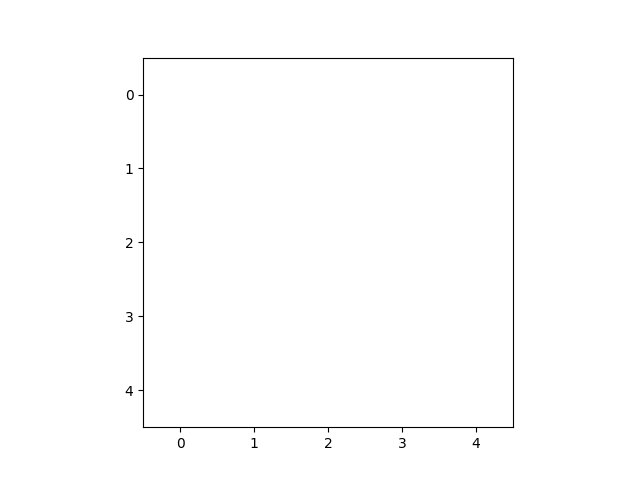
\includegraphics[width=3.5cm]{svd_approximation_0.png} \\
		\hline
		r = 1 & 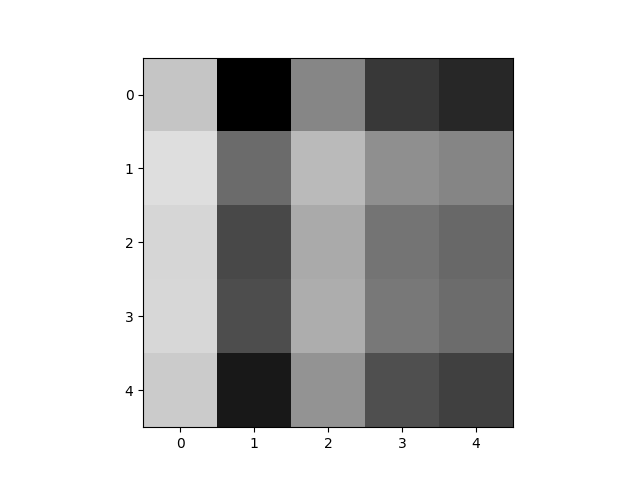
\includegraphics[width=3.5cm]{svd_approximation_1.png} \\
		\hline
		r = 2 & 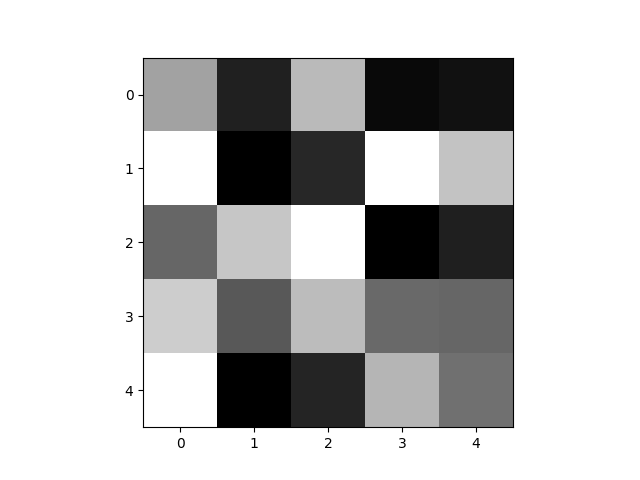
\includegraphics[width=3.5cm]{svd_approximation_2.png} \\
		\hline
	\end{tabular}
	\begin{tabular}{|c|c|}
		\hline
		Components & Approximation \\
		\hline
		r = 3 & 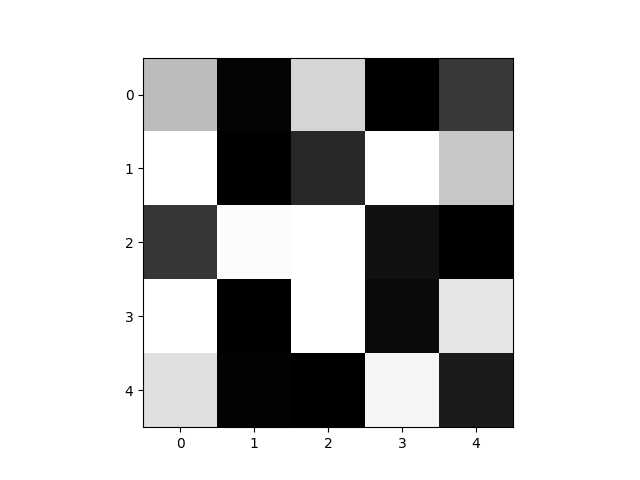
\includegraphics[width=3.5cm]{svd_approximation_3.png} \\
		\hline
		r = 4 & 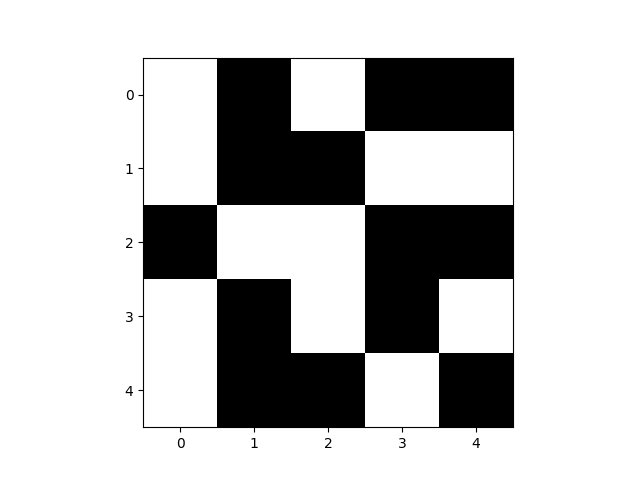
\includegraphics[width=3.5cm]{svd_approximation_4.png} \\
		\hline
		r = 5 & 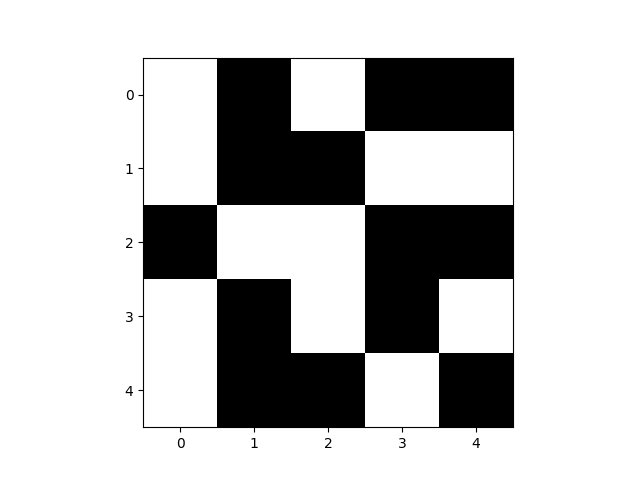
\includegraphics[width=3.5cm]{svd_approximation_5.png} \\
		\hline
	\end{tabular}
	\\\\
	When r = 1, we get a single rank-1 component of the image. You can see that each row or column is some linear combination of every other row or column respectively. That's why you get that sort of grid pattern appearing. Since the SVD can decompose a matrix into the sum of rank-1 matrices, variations of this grid like pattern, when layered on top of each other, can give us any matrix we want. 
	
	This process we've described is fine for a greyscale image, but what if we wanted to apply this to coloured images? Firstly, we need to create a test image which we will use:
	
	\begin{figure}[h]
		\centering
		\includegraphics*[width = 4cm]{test_image.png}
		\caption{Test RGB image for SVD}
	\end{figure}
	
	Each pixel in a coloured image is represented as a tuple of three integer values indicating the intensity of the red, green and blue components. This image is 200 x 300 pixels in size. Its split into three 200 x 100 segments with each part taking the maximum intensity of its respective colour. The colour of each pixel in the red section is (255, 0, 0) , (0, 255, 0) in the green section and (0, 0, 255) in the blue section. We can break this down into three images where each pixel is the intensity of the respective colour:
	\begin{figure}[h]
		\centering
		\includegraphics*[width = 13cm]{test_image_rgb_plot.png}
		\caption{RGB components of the test image}
	\end{figure}
	
	Note that each component is now a greyscale image because each pixel is only taking values between 1 and 255 inclusively. We've written some python code that can do a lot with regards to deconstructing, decomposition and plotting various approximations of any greyscale and RGB image. We won't describe how the functions work but we will include what code is needed to achieve each image. 
	
	Using the following code, we can plot 5 approximations of our RGB test image. 
	\begin{scode}
		test = image\_svd("test\_image.png") \\
		test.plot\_n\_approximations\_rgb(5) \\
		plt.show()
	\end{scode}
	The first three rows break down each colour component into increasing approximations of the matrix for that colour component. These approximations are then layered back onto each other to produce the image in the bottom row. 
	\begin{figure}[h]
		\centering
		\includegraphics*[width = 13cm]{test_image_5_components_rgb.png}
	\end{figure}
	
	One question we might want to ask about the number of components is whether we can quantify the effect of increasing the number of components with respect to how much variance of the original image is captured in every component. An important aspect of the singular value decomposition is that the singular values themselves can tell us the relative importance of each component. This is because the summand in \ref{rank_k_approximation} is weighted by each singular value. We can formalise the variance explained by each component in the following formula \cite[page 131]{mml_book}:
	
	\begin{align}
		R^2_i = \frac{s_i^2}{\sum_{j}^{} s_j^2}
	\end{align}
	
	The code we've written can plot this information for a certain number of singular values and for each RGB component. 
	\begin{scode}
		test = image\_svd("test\_image.png") \\
		test.plot\_singular\_rgb(10) \\
		plt.show()
	\end{scode} \begin{figure}[h]
		\centering
		\includegraphics*[scale = 0.65]{variance_test_image.png}
		\caption{Variance Explained for each colour component}
	\end{figure}
	
	This bar chart is for our RGB test image. You may notice that 100\% of the variance of the original image is captured in just one component. This makes sense since the test image only has a rank of 1 so all the information is contained in just the first component. Now that we've shown how our code works for a test image, we can start to experiment with some more interesting images. Consider figure \ref{fig:r_place} \cite{r_place}:
	
	\begin{figure}[h]
		\centering
		\includegraphics*[scale = 0.5]{r_place.png}
		\caption{r/place 2022 archive.}
		\label{fig:r_place}
	\end{figure}
	
	To explain this image, we need to delve into what Reddit is. Reddit is a large social media site but it functions in quite an interesting way. Anyone can go onto the site and start their own Subreddit. You can think of this as a forum specifically for that community. The community can be about (almost) anything from programming to wind turbines. If a community exists for a topic, its highly likely it is on Reddit. These individual community forums are self-regulated with their own admins and rules. One such community is the ``place" community. Every year, they run a type of social experiment where they begin with a blank 600 x 600 grid of pixels. Every 5 minutes, any Reddit user can change one pixel colour. This led to a very interesting image where each community was trying to compete for dominance on the grid. For example, there was one such ground called ``The Void" with the sole goal of turning the entire grid black. You can view a time-lapse of the most recent experiment. 
	
	Lets first take this image and look at the variance explained by each component.
	\begin{scode}
		test = image\_svd("r\_place.png") \\
		test.plot\_singular\_rgb(10) \\
		plt.show()
	\end{scode} \begin{figure}
		\centering
		\includegraphics*[width = 13cm]{r_place_sv.png}
		\caption{Scree plot for r/place image.}
	\end{figure} 
	
	I would of thought that given the complexity of the image, we might have less of the variance explained in the first component. The scree plot tells us that over 75\% of the variance of the red and green parts of the image can be explained in the first component while the blue part sits at 70\%. Lets look at what this looks like if we construct a number of computations:
	\begin{scode}
		test = image\_svd("r\_place.png") \\
		test.plot\_n\_approximations\_rgb(5) \\
		plt.show()
	\end{scode} \begin{figure}[h]
		\centering
		\includegraphics*[width = 15cm]{r_place_decomposition.png}
		\caption{Scree plot for r/place image.}
	\end{figure} 
	
	\section{Conclusion}
	In this dissertation we've discussed some of the main concepts in linear algebra required to explain a proof of the singular value decomposition for all matrices. We started by discussing what a vector space to provide an axiomatic basis for further discussions. This led into an important concept known as a linearly independent set of vectors. Following this, we explored generating sets and the span of a set of vectors, both being two sides of the same coin. This gave us a foundation for explaining the basis of a vector space. We moved onto the row rank and column rank of a matrix, providing an example to demonstrate why $ \crank{A} = dim(span[\{\matrx{A}_{.1}, \ldots, \matrx{A}_{.m}\}]) $ for any matrix $ \matrx{A} \in \real^{n \times m} $. We then went on to our first proof that $ \rrank{A} = \crank{A} $ for all $ \matrx{A} \in \real^{n \times n} $ which meant we could define a new definition, the rank of a matrix. From here, we went into the row space and column space of a matrix and at the same time, proved that the span of a set of vectors forms a vector space itself. At this point we introduced eigenvalue eigenvector pairs and determinants as a method to calculate them along with a proof of why this is the case. We proved why eigenvectors are linearly independent and why the product of eigenvalues is the determinant. This was to give the determinant a less arbitrary feeling. Following this, we proved that  $ \matrx{A}^{-1} $ exists $\iff$ $ \dett{A} \ne 0 $ using a proof by contradiction. From here, we went into linear transformations to provide an intuitive way to explain the next and main topic of the dissertation, matrix decompositions. We explained the eigenvalue decomposition along with a proof of its existence for any matrix $ \matrx{A} \in \real^{n \times n} $. This allows us to prove the existence of the singular value decomposition for any matrix $ \matrx{A} \in \real^{m \times n} $. Now that the linear algebra was laid out, we went into more practical examples of using the singular value decomposition to construct approximations of greyscale images followed by coloured images. A set of python functions was created to allow the reader to experiment with this matrix decomposition on images. 
	
	While my original goal was to build up to the singular value decomposition with a more systematized and concrete approach, it soon became apparent this wouldn't be entirely possible. I always imagined mathematics as a brick wall, building up layers of reasoning that are reliant on the previous layers with axiomatic statements at the foundations. While this is somewhat true, it doesn't help with regards to how you may explain each of these concepts. There's numerous paths that you can take to get to the same proposition and if I were to include every single brick or deduction, this dissertation would be far too long so determining what to include and what to overlook was very difficult and subjective. 
	
	It is certainly true that most example dissertations I've seen were more focused on performing some investigation with their conclusions being the findings of this investigation. I decided to focus more on a general overview of key concepts in linear algebra. Many of the proofs provided were quite difficult to understand intuitively and finding new and interesting ways to explain certain topics was what I thought would give this approach some value. 
	
	There are numerous avenues that could be taken from this work. With regards to improving the mathematical communication by using graphs, specifically networks to illustrate the connection between certain areas. I would of also liked to develop graphics to explain a long of the theory with regards to basis and generating sets. On the topic of more practical avenues of further research, I would of loved to find a way to quantify the difference between the original image and the constructed image to see if this correlates with the number of components used in the construction. Another example we didn't explore was the applications of the singular value decomposition to machine learning. the SVD can be used as a form of dimensionality reduction for high dimensional datasets while also capturing the maximum variance of the original dataset for a given number of dimensions. This means that you can train a machine learning model using less data and therefore reduce the training time. I would of loved to try and quantify this using the MNIST dataset, seeing the effect on the accuracy of the model based on this dimensionality reduction. We could of also tried to write code to perform a form of lossy compression on images, determining a suitable number of components required for an effective form of compression. 
	\printbibliography
\end{document}